
%%%%%%%%%%%%%%%%%%%%%%% file typeinst.tex %%%%%%%%%%%%%%%%%%%%%%%%%
%
% This is the LaTeX source for the instructions to authors using
% the LaTeX document class 'llncs.cls' for contributions to
% the Lecture Notes in Computer Sciences series.
% http://www.springer.com/lncs       Springer Heidelberg 2006/05/04
%
% It may be used as a template for your own input - copy it
% to a new file with a new name and use it as the basis
% for your article.
%
% NB: the document class 'llncs' has its own and detailed documentation, see
% ftp://ftp.springer.de/data/pubftp/pub/tex/latex/llncs/latex2e/llncsdoc.pdf
%
%%%%%%%%%%%%%%%%%%%%%%%%%%%%%%%%%%%%%%%%%%%%%%%%%%%%%%%%%%%%%%%%%%%


\documentclass[runningheads,a4paper]{llncs}

\usepackage{amssymb}
\setcounter{tocdepth}{3}
\usepackage{graphicx}

\usepackage{url}
\newcommand{\keywords}[1]{\par\addvspace\baselineskip
\noindent\keywordname\enspace\ignorespaces#1}

\begin{document}

\mainmatter

\title{QVT Traceability: What does it really mean?}

\titlerunning{QVT Traceability}

\author{Edward D. Willink\inst{1}
\and Nicholas Matragkas\inst{2}}
\institute{Willink Transformations Ltd., UK,\\
\email{ed-at-willink.me.uk}
\and
University of York, UK,\\
\email{nicholas.matragkas-at-york.ac.uk}}

\authorrunning{QVT Traceability: What does it really mean?}

\toctitle{Lecture Notes in Computer Science}
\tocauthor{Authors' Instructions}
\maketitle


\begin{abstract}


Traceability in Model Transformation languages supports not only post-execution analysis, but also incremental update and co-ordination of repetition. The Query/View/Transformation family of languages specify a form of traceability that unifies high and low level abstraction in declarative and imperative transformation languages. Unfortunately this aspect of the QVT specification is little more than an aspiration. We identify axioms that resolve the conflicting requirements on traceability, and provide a foundation for resolving further issues regarding equality, transformation extension and mapping refinement.
\keywords{Model Transformation, QVT, Traceability, Transformation Extension, Mapping Refinement}
\end{abstract}


\section{Introduction}

The successes of early model transformation prompted the Object Management Group (OMG) to issue a Request for Proposal for a standard solution to the problems of querying, viewing and transforming models. The initial submissions eventually converged to give us the Query/View/Transformation (QVT) family of languages. The specification standardizes research work and so the specification is imperfect.

Problems in the specification are recorded as issues that can be raised by anyone at \url{http://www.omg.org/report_issue.htm}. The issues are addressed by a Revision Task Force (RTF) that proposes and votes on resolutions. The QVT 1.2 RTF has just completed resolutions for the 125 outstanding issues against QVT 1.1\cite{QVT-1.1}. At the time of writing 2/3 have been balloted successfully, with the remaining 1/3 being voted on. However 20\% of the resolutions just agree to defer difficult issues for further consideration. This paper provides some of the further consideration and an opportunity for the wider community to comment on these issues, which while described in the context of QVT, are relevant to model transformation more generally.

In Section \ref{qvt-spec} we first summarize the specified aspects of QVT traceability, then in Section \ref{axioms} we dig down to the underlying purpose of traceability in a declarative context and formulate some axioms that enable us to consider the Object-Orientedness of transformations. The more challenging context of Imperative Transformations is discussed in Section \ref{imperative}. in Section \ref{solution} we outline a Trace Model that can be used more realistically throughout QVT. We present related work in Section \ref{related} and finally conclude in Section \ref{conclude}.

\section{QVT Traceability as Specified}\label{qvt-spec}

The QVT specification defines a family of three languages, in part reflecting differing viewpoints amongst the original submitters and in part reflecting different community requirements. 
\begin{itemize}
\item QVT Operational Mappings (QVTo) an imperative transformation language.
\item QVT Relations (QVTr) a high level declarative transformation language.
\item QVT Core (QVTc) a low level declarative transformation language.
\end{itemize}

These languages are unified via the QVTc semantics. QVTr transforms directly to QVTc. QVTo and arbitrary externally supplied blackboxes are defined with respect to an equivalent QVTr Relation. The practical compatibility of this unification has yet to be demonstrated, since the various QVTo and QVTr vendors find sufficient challenges in realizing a primary language and blackboxes without worrying about the alternative paradigm. There are no complete QVTc implementations.

In this paper we concentrate on a narrower and potentially much clearer form of compatibility; the \emph{trace record}s which are supposedly common to all three languages.

One benefit and consequence of the low level QVTc language is that the user can and must specify the
maintenance of the classes that establish traceability. These form the middle model for a typical bidirectional
QVTc mapping in which left and right hand models are related with the aid of the intermediate trace model.

A \verb|Package2Schema| mapping may therefore operate between a \verb|Package| \emph{p} and a \verb|Schema| \emph{s} maintaining a \emph{trace record} of the intermediate \verb|TPackage2Schema| \emph{trace class} with \emph{p} and \emph{s} properties.
 
\begin{verbatim}
class TPackage2Schema {
     property p : Package;
     property s : Schema;
}
\end{verbatim}

When the mapping is executed in the forward direction, the \emph{p} property is initialized with the matched input Package and the \emph{s} property with the generated output Schema. The \emph{trace instance} records the \verb|Package2Schema| relationship between \emph{p} and \emph{s} when the source-to-target relationship is first established. Thereafter another mapping can locate the schema corresponding to \verb|aPackage| by the OCL navigation \verb|aPackage.TPackage2Schema.s|, which starts at \verb|aPackage|, uses the \verb|Package::TPackage2Schema| relationship, which is the implicit opposite of the \verb|TPackage2Schema::p| relationship. This locates the \emph{trace record} and then the \verb|TPackage2Schema::s| relationship navigates to the target. This is a demonstration of the power of an explicitly modeled \emph{trace class}; there is no need for any special operators such as \verb|resolve| in QVTo or \verb|resolveTemp| in ATL.

The need for manual maintenance of the \emph{trace record}s is eliminated in QVTr for which a mapping to QVTc is suggested by Rule 1 of Clause 10.2 of the QVT specification. Unfortunately this rule neglects to specify an algorithm for construction of the trace class name and so there is no guidance on how name clashes are to be avoided.

Defining \emph{trace class}es without any common base class to support polymorphic \emph{trace instance} maintenance makes this aspect of the QVT specification totally unsuitable for practical tooling. In Section \ref{solution} we outline a more rational proposal.

The specification of QVTo \emph{trace class}es is distinctly vague since it relies on the underspecified correspondence between a QVTo MappingOperation with an unspecified Operation signature, and a QVTr Relation. Overloading is even more of a problem in QVTo with its disjuncted mappings. The need to extend the \emph{trace data} to accommodate \emph{in}/\emph{inout}/\emph{out} parameters is identified without any clarification on how the trace data is modified in a way that remains compatible with QVTc. \emph{inout} parameters present a further challenge; in QVTo an \emph{inout} parameter has distinct \emph{in} and \emph{out} values. This is incompatible with a one-to-one correspondence with a QVTr relation. QVTr is multi-directional, so a parameter may be \emph{in} or \emph{out} depending on the direction; it cannot be both \emph{in} and \emph{out}.

%We can resolve the \emph{inout} conflict by replacing each \emph{inout} parameter by an internal variable, an \emph{in} only parameter and a singly assigned \emph{out} parameter. The internal variable is initialized from the input, updated as many times as necessary and finally written once to the output.

\section{Declarative QVT Traceability Purpose}\label{axioms}

Traceability is useful to analyze the behavior of the transform when debugging or tuning, but much more importantly it enables a model transformation to transform to a graph rather than a tree. When building cross-references in the output graph, it is necessary to reference a target model element and this requires an ability to navigate the source-to-target relationships proved by the \emph{trace record}s.

\begin{figure}
  \begin{center}
    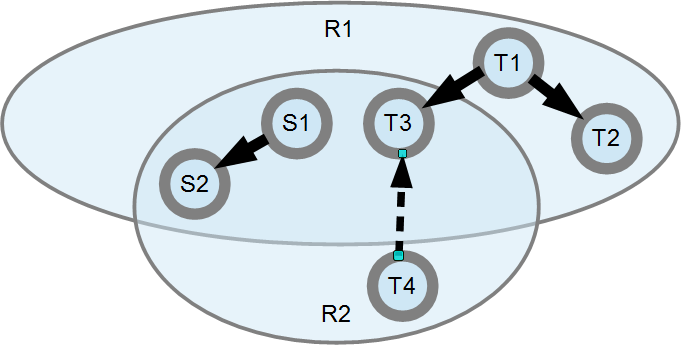
\includegraphics[width=2.0in]{Problem.png}
  \end{center}
  \caption{Target resolution Problem}
  \label{fig:Problem}
\end{figure}

Fig \ref{fig:Problem} shows the basic problem. We know that mapping R1 establishes a relationship between pairs of source model elements S1, S2 and triples of target model elements T1, T2, T3. In another mapping R2, where a similarly typed pair of source model elements S1, S2 reoccurs, we require to re-reference one of R1's target model elements, T3, in order to establish a cross-reference from T4. We can solve this problem if we maintain \emph{trace data} comprising a \emph{trace record} that relates the tuple (R1,S1,S2) to the tuple (T1,T2,T3). We then just ask the \emph{trace data} to return the appropriate (T1,T2,T3) for our new relationship R2 where we want to know about (R1,S1,S2) model elements.

We will now examine what properties we need traceability to exhibit in order to perform declarative transformations. Once we understand declarative transformations, we can then see in Section \ref{imperative}, how the QVTo imperative transformation language can conform to the same principles.

\subsection{Trace Record Axioms}

\subsubsection{Trace Representation}

A \emph{trace representation} summarizes the state of an input or an output model element.

The \emph{trace representation}s of any pair of model elements contains sufficient information to determine whether the two model elements are equal. Additionally an \emph{output trace representation} contains sufficient content to allow the represented element to be reconstructed.

UML, and consequently OCL and transformation languages based on UML or OCL, define two importantly different forms of model element.

Each Class instance or object represents a distinct model element; no two objects are ever equal. It is therefore convenient to summarize the state of any object by its memory address since each object has a distinct address. Reconstruction of the object from the summary is trivial, so long as the object remains in memory.

An instance of a DataType (such as Integer or a Collection(String)) has a value. Instances of DataTypes are equal when they have the same value, even if the instances are stored at distinct addresses. 4 is clearly always equal to 4 no matter what address the 4 is at. 
%In OCL (unlike Java), the string  `four' is also always equal to `four'.
For values such as Integers, whose storage requirements are small, it is convenient to use the entire value as the representation. For potentially very large values such as Strings or Collections, it is convenient to use the address as the summary, making reconstruction easy, but requiring care to compare the underlying value rather than just the \emph{trace representation} when determining whether two DataType values are equal.

\subsubsection{Trace Record}

A \emph{trace record}, which may also be called a \emph{trace instance} of a \emph{trace class}, comprises
\begin{itemize}
\item the identity of the mapping that is traced
\item an ordered list of the \emph{input trace representation}s of each mapping input argument
\item an ordered list of the \emph{output trace representation}s of each mapping output result
\end{itemize}

(The ordering of the lists may be established by some deterministic algorithm such as an alphabetic sort applied to the names of the mapping parameters.)

\subsubsection{Trace Identity}

A \emph{trace identity} comprises the first two elements of the trace record; mapping identity and \emph{input trace representation}s.

\subsubsection{Trace Identity Uniqueness}

No two \emph{trace record}s share the same \emph{trace identity}.

\subsubsection{Trace Data}

The \emph{trace data} comprises all the \emph{trace record}s.

\subsubsection{Trace Record Creation}

Every mapping execution has a \emph{trace identity} and a corresponding \emph{trace record}.

Consequently any attempt to execute a mapping that would require a duplicate \emph{trace identity} must be detected and suppressed. The results  of the suppressed execution are reconstructed from the \emph{output trace representation}s of the previous execution.

\subsubsection{Trace Record Access}

The \emph{trace data} may be exploited to recover a \emph{trace record} for a given \emph{trace identity} and so locate the target for a graph-to-graph transformation.

Consequently the \emph{output trace representation} must be consistently determined by the \emph{trace identity}.

If an underlying input model element changes, then the \emph{input trace representation} changes too and so the mapping must be re-executed if the corresponding outputs are required.

\subsection{Tracing immutable Class instances and DataType values}

With distinct input and output models, the input model elements may be stable for a declarative transformation or a well-behaved imperative transformation and so the use of an address to summarize each unchanging object is valid.

Maintaining a \emph{trace record} for immutable DataType or Class instances therefore just requires the address of the relevant instance to be retained. This incurs very limited cost apart from limiting Garbage Collection in long running programs.

%Essential OCL is a side-effect free language that can query the unchanging state of a modeled system\footnote{Complete OCL adds the @pre operator to support queries involving two (pre and post) states of a system.}. All DataType values and Class instances are therefore immutable.

\subsection{Tracing mutable Class instances and DataType values}

However for an in-place transformation or less well-behaved imperative transformation, model elements may be updated requiring a more complete \emph{input trace representation} to ensure that the mapping is executed again for a changed input to yield a correspondingly changed output.

For in-place declarative transformations, it may be possible to treat the transformation as an out-of-place transformation followed by a copy back to the input so that all changes are localized in the copy-back.


\subsection{Child Stealing}

Access to previous results is necessary to be able to resolve the targets in graph-to-graph transformations. The declarative formulation, as replacement of the result of a mapping re-execution by the original results, can have an unpleasant corollary if those graphs are UML or Ecore models with composition relationships. A composition relationship imposes a limitation that a model element can only be in one container. Consequently a conflict arises when a model element, that already is already the target of one composition relationship, is assigned as the target of another composition relationship.

The problem is demonstrated by the following example in which the intent is to transform an incoming model comprising a single \verb|Node| instance, into a model comprising a \verb|Node| instance with 10 composed child \verb|Node| instances and a list of 10 references, one to each child \verb|Node|. 

\begin{figure}
  \begin{center}
    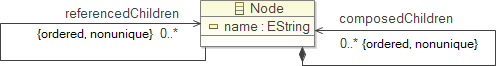
\includegraphics[width=3.25in]{ChildStealingMM.png}
  \end{center}
  \caption{Metamodel for the child-stealing example}
  \label{fig:CSMM}
\end{figure}

However when we execute the transformation, we get a \verb|Node| instance with a single child \verb|Node| and a list with 10 references to the one child.

\begin{figure}
  \begin{center}
    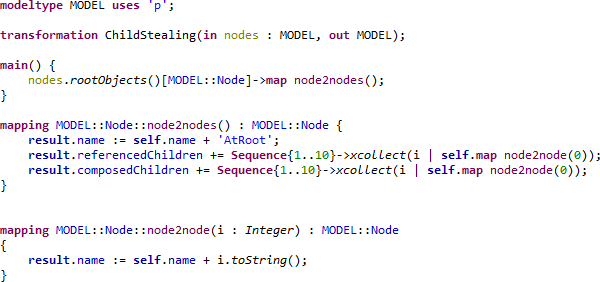
\includegraphics[width=4.75in]{ChildStealingCode.png}
  \end{center}
  \caption{QVTo Code for the child-stealing example}
  \label{fig:CSCode}
\end{figure}

The critical part of the code is \verb?Sequence{1..10}->xcollect(i? that arranges for \verb|i| to loop over the integers 1 to 10 and collect the results of a \verb|self.map node2node(0)| mapping invocation at each loop iteration. The first invocation of the mapping creates a new \verb|Node| as required, but subsequent invocations have the same \verb|(node2node,self,0)| \emph{trace identity} and so return the existing \verb|Node|. The collected results therefore comprise the same result ten times and when \verb|result.composedChildren += | assigns them to a composition, the first assignment succeeds and each subsequent assignment re-assigns.

Users of the Java API for EMF\cite{emf} will be familiar with the confusing disappearance of elements from containers because they were reassigned to alternative containers in seemingly totally unrelated code. For Java programmers, this may be an unavoidable consequence of low level practices. For an imperative transformation language the surprising non-local side effects are very undesirable, but can at least be predictably located when single stepping. For a declarative transformation language, there is no clear schedule and so the surprise may be dependent on the accidental ordering of mappings executions; this cannot be acceptable.

We have a conflict between traceability-driven re-use and composition; the results that the \emph{trace record} gives us for re-use are not fit for exclusive re-use. The problem is that the \emph{trace identity} has insufficient discrimination to exclude alternative re-use. In the example above the tuple \verb|(node2node,| \verb|self:Node,| \verb|i:Integer)| is adequate but the calling code always uses 0 as the Integer provoking the unwanted re-use. Changing the caller to pass the loop `counter' to the mapping makes the usage exclusive and we get the desired 10 \verb|composedChildren|.

We can see that Child Stealing is a serious problem and we can easily detect it. During normal execution each model element is created without a container and then assigned to a container. It is very rare for model elements to be intentionally re-assigned to another container, so we can define any such re-assignment as a Child Stealing Error. If there is a real requirement for re-assignment, we can require that  it is performed in two stages, first to explicitly de-assign the container before re-assigning. In some cases it may be possible to detect Child Stealing Errors by static analysis.

%For a complex object, it may be stupid to require a duplicate, but for simple objects it may be very reasonable. For instance a model user might have a Item that can be contained by a ShoppingBag or a StockRoom mapping. If the Item contains an ItemName that has a String value and the ItemName is created by a String2ItemName mapping, ItemName instances may be shared causing some Items to lose their name. Worse, with ItemName no longer reliable, if I put an Item in my ShoppingBag, it may remove an inadvertently shared Item from your ShoppingBag or the StockRoom. The application is not inherently faulty, it is as reasonable to have many ItemName objects with the same name as to have physical labels with the same writing on. The problem is the inadvertent imposition that labels are managed by a clever traceability system that prohibits duplicates.

%Since the permitted duplication is a semantic issue that is not properly modeled, it does not seem likely that a satisfactory algorithm can diagnose the hazard so that the model or transformation can be adjusted.

%Prohibiting duplicates does not seem to be an option, so how can we handle them? Since traceability automatically suppresses all duplication, perhaps the provision a re-usable result should ensure that the result is fit for re-use. 

%This could mean automatic and immediate creation of a deep-clone, but for objects, this may cause downstream confusion because the deep-clone may have a different address and so fail to share the \emph{trace identity} for a subsequent mapping. 

%Perhaps we introduce a LazyClone<T> to wrap a T object so that we have a distinct object to satisfy the containment but have an object that is able to delegate its identity to the original object. This may cause difficulties for type conformance since LazyClone<T> is not a T and T might be a final class prohibiting derivations.

%The above approaches are attempting to support graph-to-graph transformation in an environment in which the target graph cannot be an arbitrary graph; sharing must be eliminated from any shared containment.

%\emph{Containment is in conflict with traceability}.

%Do we need traceability with unique \emph{trace-identity} restrictions rather just than a simple execution recording?

%In an imperative language such as QVTo, traceability can be simulated with a manually maintained Dict that is passed through the explicitly scheduled mappings, so traceability could be discarded.

%However in a declarative transformation language we have many relatively isolated relations with no inherent intercommunication and certainly no ability to accumulate intermediate results. It is only the data dependencies that impose limits on the scheduling, and traceability is the ability to interrogate the consequence of a data dependency. Traceability seems unavoidable.

%Do we need containment? While performing the transformation we could use model representations in which containment was ignored and only re-instate containment by creating deep-clones when presenting the output graph as a conformant model to another tool or for serialization in XMI. Conversely when reloading from another tool or from XMI, we must merge all source objects that are indistinguishable. This is not particularly helpful for in-place transformations where we would like to use the true objects. We can solve this problem by distinguishing true-objects and traceable-objects and maintaining an N:1 mapping between the N true-objects and the 1 traceable-object; transformation startup creates the N:1 mapping transformation execution updates a containment-free graph of traceable-objects and finally transformation completion reverses the 1:N mapping to distribute each traceable-object content to each true-object.

%How do we manage without containment? Containment provides us with a tree structure that is convenient in many ways, not least of which is imposing some order on an XML serialization. Containment and tree-structure are fundamental to EMF and EMF forms the foundation of many/most modeling tools, so eliminating containment without revising EMF is a challenge.

%If our tooling uses models reified as Java code or any user defined Java enrichment, it may be very difficult if not impossible to bypass the unwanted containment imposition.

%However, if our tooling uses only EMF models and avoids and any generated Java code, we may clone the user metamodel, reset the containment relationships and use the containment-free metamodel within our tooling. A metamodel enriched with OCL operations may be used provided the OCL makes no attempt to invoke oclContainer(). We will need a model loader that shares duplicates, and an unloader that recreates them.

%Alternatively once we have lost the ability to support Java-defined model enrichment, we may move to a custom internal model representation that supports only the facilities necessary for model transformation and so bypass the overheads that EMF's power and flexibility impose.

\subsection{Transformation Extension and Mapping Refinement}

All three QVT languages define transformations that may extend other transformations, and mappings that may refine other mappings, but neglect to define what this may mean. The immediate question is are transformations Object-Oriented and do they observe the Liskov Substitution Principle\cite{liskovSubstitutionPrinciple}? 

We would very much like transformations to be Object-Oriented so that we can use familiar derive and override practices, so let us assume a strong analogy between the new Transformation/Extension/Mapping/Refinement concepts and the familiar Class/Inheritance/Operation/Overriding. We will exploit the traceability axioms to see what limitations we may need.

The Liskov Substitution Principle is of course never observed unequivocally, but disciplined transformation writers can define those behaviors for which substitutability is important and code their refinements accordingly.

\subsubsection{Transformation Extension}

For the model parameters of an extended transformation, we might look for an analogy with the arguments of a derived constructor, where the arguments can be very different and must be converted to use one of the inherited constructors. However for transformations there is just a single interface of one model-type per model-parameter and there are no conversion facilities. A model-type is a list of packages of types that the transformation compiler needs to consider; the model-type is not significant at run-time. The transformation extension therefore just routes the models of the extending transformation to the extended transformation. Since the execution direction is unknown, every type that could be generated by the extended transformation must be included by the model-type of the extending transformation, so we require:

\emph{All extending transformation model-types must be super-sets of the extended model-types}. 

\subsubsection{Mapping Refinement}

The declarative QVT languages are multi-directional and so we do not know which mapping parameters are inputs and outputs. There is therefore no opportunity for covariant or contra-variant refined mapping parameter types.

\emph{Refining mappings must overload the refined mapping signature without change}.

\subsubsection{Dynamic Dispatch}

For OO-style dynamic dispatch of mappings to work, we require:

\emph{QVTc and QVTr must have a this object that is an instance of the executing transformation}. 

The instance can be stateless. 
%For QVTo, a transformation is an object whose features may be exploited using the reserved \emph{this} variable. QVTc and QVTr provide fewer transformation capabilities and so have no need of a \emph{this}, however as we shall see the concept of \emph{this} as a stateless instance identifying the current transformation is useful in QVTc and QVTr as well.

%A typical use case for transformation extension might I arise if I decide that your transformation from UML2Doc is very useful but I want to extend it for use with BigUML. If transformation extension is little more than a package import to make names accessible, then my BigUML2Doc can exploit UML2Doc but no UML2Doc functionality can be overridden, unless the UML2Doc author has anticipated extension by incorporating some non-standard join-point capability. In contrast, if transformation extension is similar to object inheritance, then mapping refinement is similar to operation overriding and my BigUML2Doc transformation can override any UML2Doc mapping whose functionality is unsuitable. This can only work if mappings are dynamically dispatched on the actual \emph{this} transformation type. Therefore a QVTo mapping declared as 

%\begin{verbatim}
%mapping Package::packageToChapter() : Chapter
%\end{verbatim}

%has hidden first, second and last arguments. An equivalent longhand OO-style declaration might be:

%\begin{verbatim}
%mapping UML2Doc::packageToChapter(in self : Package, out result : Chapter)
%\end{verbatim}

%with an override

%\begin{verbatim}
%mapping BigUML2Doc::packageToChapter(in self : Package, out result : Chapter)
%\end{verbatim}
 
%In QVTo the direction is known, so contravariant output types might be possible. However QVTr and QVTc are multi-directional so while QVTo mappings have a QVTr relation correspondence QVTo mapping arguments must be type invariant.

\subsubsection{Tracing}

When we consider a \emph{trace record} involving execution of  a refined mapping, should the apparent invoked mapping or the actual executed mapping be recorded? A subsequent user of the trace must be able to resolve against the apparent mapping, rather than all possible refinements, but must also be able to resolve against the actual mapping where that is known. 

\emph{There must be a trace record for each possible trace identity}.

This does not necessarily imply multiple \emph{trace record}s and in Section \ref{solution} we propose to allow a \emph{trace record} to have multiple \emph{trace identities}.

\subsubsection{Composition}

An overridden declarative mapping provides a composition of predicates and assignments.

In accordance with Design by Contract\cite{dBc} all predicates should be satisfied. There may obviously be scope for optimization of redundancy.

Similarly all assignments should be made, but since multiple assignments may conflict, each most derived assignment should be chosen, thereby allowing a refining mapping to adjust as well as extend the behaviour of a refined mapping.

\emph{A mapping refinement hierarchy is equivalent to a single composite mapping}.

%If we consider a large system in which the BigUML2Doc invokes a nested execution of EvenBiggerUML2Doc either of which override the  UML2Doc::commentToNote mapping, should the two transformations share the trace records for commentToNote mapping executions? If we had to worry about child stealing, we would have to totally isolate the two transformations to avoid anarchy. With child stealing solved by auto-deep-cloning, we can continue to exploit the ability of a trace record to ensure that repeated mapping invocations are suppressed in favor of re-use.

%If we record the apparent invoked mapping, then different overloads/refinements would share the same trace identity. The trace record must therefore record the actual mapping and avoid interference when the same model elements are used in different transformations with different refinements.

\subsubsection{Concurrency}

If we have a system in which more than one copy of a transformation executes on the same input models, we may want to share common model elements but must keep composed model elements exclusive. Providing a single overall \emph{trace data} will satisfactorily share the common model elements, but we must avoid Child Stealing of the exclusive model elements. Most mappings create composed children with the intended parent as one of the traced inputs, so provided the parents are exclusive, the children will be too. We therefore only need to ensure that the root parent is exclusive, which may be achieved by using the transformation \emph{this} as part of the \emph{trace identity}.

 \emph{Trace data may be shared by concurrent transformations}.
 
This same reasoning applies to the nested execution of extended/extending transformations or refined/refining mappings.

\section{Imperative Traceability}\label{imperative}

So far we have concentrated on the declarative QVT languages where the ability for objects to mutate and the ability to impose a schedule is very limited. Declarative scheduling is an implicit consequence of the inability to perform a mapping until its inputs are available. Complex input/output dependencies may result in the mappings being grouped into passes. Object mutation is limited to one value at the input/output of each `pass'.

\subsection{Imperative Characteristics}

In contrast QVTo allows the user to
\begin{itemize}
\item specify an explicit execution order
\item make arbitrary changes to objects
\item use mutable collections
\item exploit changeable global context
\item exploit changeable transformation context
\item have \emph{inout} mapping arguments
\end{itemize}

Of these only the explicit order is not a problem for traceability; it just allows an infeasible order to be programmed.

\subsubsection{Object changes}

If an object changes, the result obtained from a mapping execution using that object prior to the change may not be valid and so the assumption that its state can be summarized by just its address is unsound; the \emph{input trace representation} must be extended to all mutable fields that influence the mapping execution. This may be difficult to determine when complex helper functions are used, so it may be necessary for the \emph{input trace representation} to create a deep-clone of the traced input unless an existing deep-clone can be re-used.

%Consider a simple class Name with a String value and a Name2UppercaseName mapping. The mapping is first executed on Name(`me') to yield UppercaseName(`ME'). If the content of the source object is now changed to Name(`you') and we consult the traceability to discover the corresponding object-to-object equivalence and so get UppercaseName(`ME') or should the traceability require the mapping to be re-executed to give the object-content-to-object-content equivalence and the result UppercaseName(`YOU')?  Of course it should be the latter, but that is very expensive so ...

The \emph{trace record} must also maintain a deep-clone of the output in order to avoid any corruption by user assignments, but this makes it impossible to return the same result as a previous mapping execution, since each new result must be a clone to avoid corruption by assignments.

\subsubsection{Collection changes}

QVTo introduces two new forms of mutable collection: List and Dict. These are very convenient for imperative programming, but have never been fully characterized in terms of their UML alignment. Is List\{1\} equal to List\{1\}? Obviously Yes. Is List\{2\} equal to List\{1\}? Obviously Not, not even if List\{2\} arose from changing List\{1\}. List is therefore clearly a Mutable DataType whose  memory location is irrelevant since only its value is interesting.

This therefore presents the same problem as for Object changes. The \emph{input trace representation} and \emph{output trace representation} must be deep-clones to avoid value corruption in the \emph{trace record}.

\subsubsection{Global context changes}

The global context such as configuration properties may influence the mapping execution and the global context may be changed between mapping executions. It is therefore necessary to include the prevailing state of all relevant mutable global context as part of the \emph{trace identity} in order to accurately determine whether the previous mapping execution result can be re-used.

\subsubsection{Transformation context changes}

Transformation context such as contextual properties and intermediate classes may also influence the mapping execution and again this context may be changed between or during executions. It is therefore also necessary to include the prevailing state of all relevant mutable transformation context as part of the \emph{trace identity}.

\subsubsection{Mapping argument changes}

A QVTo mapping may have \emph{inout} arguments which may influence the behavior, so we should deep-clone the relevant parts of the value on input as one of the \emph{input trace representation}s and the whole output as one of the \emph{output trace representation}s.

\subsection{Assessment}

It may be noted that all this additional context is also required to fulfill the goal that the trace record contains the information necessary to determine what needs to be re-executed as part of an incremental update.

QVTo is intended to be a practical language, so introducing all the additional \emph{trace record} content identified above to make traceability sound seems unacceptable. The cost of all the deep-cloning is obviously large and may be quadratically so. Consider a relatively simple mapping in which the programmer either does not understand, or does not trust, the built-in \emph{trace record} resolution capabilities. An \emph{inout} Dict is passed in order to keep track of all the input to output mappings. This Dict will grow in size with each mapping and so we have a steadily growing Dict to deep-clone and consequently O(N*N) complexity.

We must instead try to tighten to the language to retain utility while adding some integrity.

The major problems of deep-cloning to stabilize the \emph{trace identity} can be avoided if all traced inputs are transitively immutable. This can be achieved for inputs by requiring an \emph{in} rather than \emph{inout} parameter and introducing a new restriction that only constants, exclusive clones or \emph{in} parameters may be passed to \emph{in} parameters. This guarantees that \emph{in} can be used without deep-cloning.

A similar policy could be applied to outputs, but the language would be useless; it would be impossible to execute a mapping to create a parent object and then populate its children, either in the caller or in a separate piece of code that uses the trace to resolve the output for update in a second pass. It seems necessary to allow the \emph{output trace representation} to evolve.

Changes to the global context can be ignored, in the hope that users will restrict the use of global context to stable configuration that requires a total re-evaluation for any change. It may be possible for tooling to detect global context sensitivity and guide users into refactoring their transformation so that unstable global context becomes a disciplined input model.  

Some changes to the transformation context could be similarly ignored, but the transformation itself cannot. There is no way that two concurrent imperative transformations operating on the same models can safely share mapping execution outputs. The transformation \emph{this} must therefore form part of an overall \emph{trace identity} or distinct \emph{trace data} must be maintained for each transformation execution.

\emph{inout} arguments must also be ignored in the hope that their usage is to accumulate additional information that does not influence the mapping execution result. This is true of the user-maintained traceability example above. It may often be possible to verify this statically, but not always. We may perhaps be able to impose a transitive prohibition on an \emph{in} or \emph{out} argument ever being used as an \emph{inout} argument.




%Maintaining a trace record for a Mutable DataType is not so simple, since if we maintain just a reference to a memory location, the value may be changed by another usage of that memory location invalidating the trace record. Mutable DataTypes must therefore be deep-cloned in order to participate reliably in detected whether a mapping invocation repeats a previous mapping invocation and should therefore return the previous results.This requirement for a deep-clone applies to Mutable DataType returns as well since they too might otherwise experience unwanted mutation. 

%Maintaining clones of Mutable DataTypes for the trace will therefore incur at least a proportionate cost to create the deep-clones. However for a relatively simple mapping in which the programmer either does not understand or does not trust the built-in trace record resolution capabilities, the cost may be quadratic. Consider a mapping in which a Dict is passed in order to keep track of all the input to output mappings. This Dict will grow in size with each mapping and so we have steadily increasing Dicts to clone and consequently O(N*N) complexity.

%The simplest solution would be to just prohibit all usage of Mutable DataTypes in mappings. However this detracts significantly from the language utility and just forces the hard-to-analyze use of global variables as a workaround. Alternatively users can convert Mutable DataTypes to an immutable form and incur exactly the same deep-cloning costs explicitly rather than implicitly. 

%More practically we can prohibit the usage of Mutable DataTypes in trace records. We can recognize that inout parameters to mappings are not useful and must be replaced by distinct in and out contributions in the trace record. We could therefore re-define inout mapping parameters as untraced.
%This retains the ability to pass information into and out of the mapping at the expense of a hazard that the mapping is influenced by the untraced parameters. This hazard can be mitigated by static analysis to confirm that the out parameters are independent of the inout parameters. The hazard cannot be avoided, since total program analysis may be necessary to conform that a linearly increasing object identity is indeed used only for identity or diagnostic purposes.

\subsection{Transformation Extension and Mapping Refinement}

The declarations of QVTo's OperationalTransformation and MappingOperation have many similarities to the declarative Transformation and Mapping so we may look to achieve Object Oriented behavior for imperative transformations as well.

QVTo provides additional mapping refinement options.

A \emph{disjunct} mapping provides an outer mapping which redirects to one of a number of inner mappings according to a type and guard-based selection. Since the outer mapping performs no object creation, the \emph{trace record} for a disjunct mapping can be provided by the selected inner mapping, augmented by the additional  \emph{trace identity} of the also-executed outer mapping.

An \emph{inherited} mapping creates an object in the outer mapping before the inherited inner mapping initializes it and returns control for further execution by the outer mapping. Since the outer mapping performs the object creation, the \emph{trace record} for an inherited mapping can be provided by the outer mapping, augmented by the additional  \emph{trace identity} of the also-executed inner mapping.

A \emph{merged} mapping executes an outer mapping then executes an inner mapping. Since the outer mapping performs the object creation, the \emph{trace record} for an inherited mapping can be provided by the outer mapping, augmented by the additional  \emph{trace identity} of the also-executed inner mapping.

%Trace data is maintained throughout the execution of a transformation. It ensures that no mapping is executed more that once for each distinct tuple off its inputs, that repeated executions with the same tuple of inputs yield re-use the precomputed outputs and enables resolve operations to interrogate the mappings. The trace data may facilitate incremental update of outputs in response to input changes. The trace data may also form an additional transformation output to enable the operation of a transformation to be analyzed or debugged.

%Trace classes

%QVT Core maintains trace data explicitly by QVT Core, while QVT Operational and QVT Relations maintain trace data implicitly. Trace data comprises instances of trace classes for which Rule 1 of Clause 10.2 defines the synthesis of a trace class from eachRelation with a property for each pattern variable. The trace class for an OperationalTransformation is  a trace class is created The transformation trace class for an OperationalTransformation trace class is created. The mapping trace class for a MappingOperation is  a trace class is created
%in .... inout Tname_in-alias1_in-alias2 ....

%Trace Creation

%For a simple MappingOperation, the \emph{trace instance} is created during execution of the initialization section of the mapping where all inputs and outputs are known but before any other mappings are invoked.

% For a blackbox transformations, the \emph{trace instance} is created and the in-properties are populated before the blackbox starts. The out-properties are populated when the blackbox completes.

%For a Relation, the \emph{trace instance} is maintained by the Relation.

%For an accessed OperationalTransformation, a transformation \emph{trace instance} .

%For a disjuncted mapping, a distinct \emph{trace instance} is created for the disjuncting mapping and for the chosen disjuncted mapping.

%For a disjuncted or inherited mapping, a distinct \emph{trace instance} is created for each disjuncted/disjuncting and each inherited/inheriting mapping.

\subsection{Incremental Update}

The QVT specification mentions the utility of the \emph{trace data} to support efficient incremental update. This may be supported by QVTc and consequently QVTr, but is certainly not for QVTo as specified.

QVTo specifies that a \emph{trace record} is created during the object initialization phase, which occurs after guards have been evaluated. Consequently there is no trace of model elements that were not created and so it is difficult for an incremental update to correctly handle a change that affects the execution of the guards.

QVTo provides no \emph{trace record} for explicit object creation or for explicit cloning.

These limitations in conjunction with the pragmatic exclusion of global, transformation and \emph{inout} context from the \emph{trace record} suggest that in order to achieve reliable incremental update with QVTo, it may be necessary to impose so many declarative characteristics that it may be more profitable to develop a QVTo to QVTr migration assistant than an incremental QVTo solution. 

\section{Multi-language solution}\label{solution}

In Section \ref{qvt-spec} we identified the strong bias of the QVT specification trace model to QVTc. In Figure \ref{fig:TraceDataMM} we suggest a more flexible metamodel that avoids imposing enumerated QVTc-style trace classes on QVTo, supports polymorphic access to the trace and provides for extension to support specialized tracing of specialized mappings such as QVTo disjuncts. 
\begin{figure}
  \begin{center}
    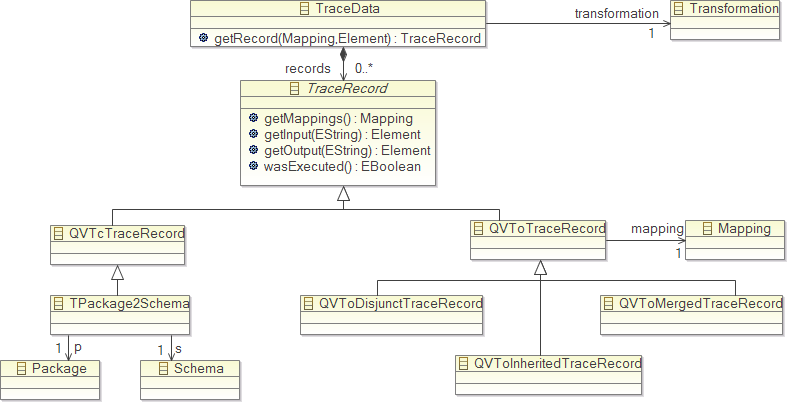
\includegraphics[width=4.5in]{TraceData.png}
  \end{center}
  \caption{Metamodel for the Trace Data solution}
  \label{fig:TraceDataMM}
\end{figure}

The abstract \verb|TraceRecord| provides the freedom for \verb|QVTcTraceRecord| and \verb|QVToTraceRecord| to pursue different representation strategies.

The \verb|TPackage2Schema| is an example of an enumerated QVTc trace class. Apart from the inheritance, it is exactly what, and all that, the QVT specification defines.

The \verb|TraceData::getMapping| API supports discovery of a trace record for a given  \verb|Mapping| operation and list of  \verb|Element|s. The  \verb|TraceRecord::getMappings| provides the list of all  \verb|Mapping| operations executed.  \verb|TraceRecord::getInput| or  \verb|getOutput| enable a particular input or output model element to be recovered.  \verb|TraceRecord::wasExecuted| enables additional tracing of unexecuted mappings to be recorded to support incremental update. 

\section{Related Work}\label{related}

In the context of model transformation, traceability can be used in a variety of
scenarios such as impact analysis or object resolution. Due to this the majority
of model transformation languages provide direct or indirect support for
tracing.

The Atlas Transformation Language (ATL) \cite{jouault2006transforming} uses
tracing to resolve the interactions and dependencies between the rules of a
transformation. The traceability mechanism offered by ATL is implicit, in the
sense that the tracing information is captured automatically by the
transformation engine without any input or guidance from the end user.  Every
time a transformation rule is matched, a new trace link object is created
between the source element and its corresponding target element(s) by using the
native type \emph{ASMTransientLink}. This trace link is assigned the name of the
rule, the source and target elements, and it is added to a link collection named
\emph{ASMTransientLinkSet}. This link collection is used internally by the ATL
virtual machine and it is not directly accessible by the end user. ATL provides
the \emph{resolveTemp()} method, which makes possible to point from an ATL
transformation rule to any of the target model elements by using the name of a
model element. One limitation of this approach is that the end user does not
have richer access to the traceability information. For example, searching by
type or iterating over all trace links is not supported. \cite{yie2009advanced}
propose a method that allows richer run-time access to traceability information
by extending the \emph{ASMTransientLink} and \emph{ASMTransientLinkSet} classes.
A second limitation of the ATL traceability support is the fact that after the
execution of the transformation the traceability information is discarded. In
\cite{jouault2005loosely} the authors propose a method for persisting
traceability information. In this method traceability-specific code is embedded
in the transformation code. When a transformation is executed this code
generates a traceability model. The traceability-specific code can be added
either manually or by the use of a Higher Order Transformation (HOT).  Although
the proposed solution solves the problem of persistence of traceability
information, it creates an overhead problem.


Another transformation language, which provides direct support for traceability,
is the Epsilon Transformation Language (ETL) \cite{kolovos2008epsilon}.
Similarly to ATL, ETL uses traceability for resolution of source elements in the
target models during a transformation execution. ETL traceability is implicit.
When a rule is matched, the ETL engine generates an instance of a
\emph{Transformation} class. This instance captures the source element of the
rule, a collection of the target elements, and the rule, which was used to
create this trace. Once a trace  is created it is added to the
\emph{TransformationTrace} object, which holds a collection of Traces for a
particular transformation. ETL provides the \emph{equivalent()} built-in
operation, which uses the generated trace links  to automatically resolve source
elements to their transformed counterparts. When the equivalent() operation is
applied on a single source element, it inspects the established transformation
trace and invokes the applicable rules (if necessary) to calculate the
counterparts of the element in the target model. Epsilon defines a set of model
management Ant tasks for orchestration workflows. One of the provided tasks is
the \emph{ETLTask}, whose exportTransformationTrace attribute  enables
developers to export an internal transformation trace to the project context.
Finally, ETL supports rule inheritance. When a rule extends another rule, the
ETL engine keeps only the sub-rule as part of the trace, ignoring the
super-rule.

In Kermeta, a traceability framework for facilitating  the trace of model
transformations is defined \cite{falleri2006towards}.The framework is built atop
a language independent traceability metamodel. In Kermeta, a model
transformation trace is defined as a bipartite graph with source and target
nodes. To support transformation chains, Kermeta defines every trace as an
ordered set of trace steps, each of them representing a single transformation. A
trace step can consist of many links, which relate source and target objects. To
generate trace information during the execution of a Kermeta transformation,
traceability-specific code has to be embedded in the transformation code.
Finally, the generated trace links can be serialized and subsequently used in
further model management tasks.


In the Simple Transformer (SiTra) tool, traceability is inspired by the
traceability support of QVT. Tracing consists of the \emph{ITrace} interface,
which holds a collection of \emph{TraceInstances}. Each trace represents a
mapping between a source and a target model element through a transformation
rule. An implementation of the \emph{ITrace} interface provides a number of
methods to query the trace collection and return all target instances. The Sitra
transformation engine ensures that, for each transformation rule being executed,
a trace is recorded.

In the context of QVT, \cite{aranega2011using}  argue that the trace mechanism
of the QVT Operational does not capture enough information for common scenarios
requiring traceability as input. To enrich the information content of this
trace, they propose an alternative metamodel which can be used in conjunction
with QVT and it can support richer traceability models.

In the approaches presented so far, there is dedicated support for the creation
and usage of traceability. In addition to the aforementioned model
transformation languages, there are other languages which do not support
directly traceability such as AGG \cite{taentzer2004agg}, VIATRA
\cite{varro2003viatra} and GReAT \cite{agrawal2003graph}. Such approaches can
support traceability indirectly by creating and manipulating trace links as any
other element.

\section{Conclusion}\label{conclude}

We have identified the intent that a single form of traceability should be shared across the family of QVT languages in order to avoid repeated mapping execution and found this to be incompatible with the current specification.

We formulated the intent of traceability as axioms and identified a potential conflict with composition relationships leading to the Child Stealing phenomenon. We have used the axioms to clarify the semantics of transformation extension, mapping refinement, tracing and concurrency in a declarative context.

We have identified significant limitations in the ability to trace reliably in an imperative context and proposed limitations that QVTo could impose to improve tracing integrity.

\subsubsection{Acknowledgments}

Thanks to Adolfo Sanchez-Barbudo Herrera for some helpful comments on an early draft.

\bibliographystyle{abbrv}
\bibliography{QVTtraceability}

\end{document}
